\documentclass[10pt,a4paper]{article}
\usepackage[utf8x]{inputenc}
\usepackage{ucs}
\usepackage{amsmath}
\usepackage{amsfonts}
\usepackage{amssymb}
\usepackage{makeidx}
\usepackage{listings}
\usepackage{graphicx}
\usepackage{inputenc}
\usepackage{makeidx}
\usepackage[german]{babel}
\usepackage[T1]{fontenc}
\usepackage{hyperref}
\renewcommand{\familydefault}{\sfdefault}
\usepackage{helvet}
\makeindex
\author{Simon Groth}
\title{Anleitung zur Erstellung eines Plug-ins für Alvis}
\begin{document}

\maketitle

\tableofcontents

\section{Einleitung}
Ein Plug-in dient dazu das Alvis-Programm zur Visualisierung von Algorithmen um weitere Algorithmen-Typen zu erweitern. Die Algorithmen werden von dem Benutzer des Programms definiert. Daher muss das Plug-in die Datentypen, welche für eine bestimmte Algorithmenart benötigt werden liefern. Außerdem die Möglichkeit diese Datentypen zu erstellen und zu visualisieren.
\section{Vorkenntnisse}
\begin{list}{-}{Sie sollten über diese Kenntnisse verfügen.}
\item Entwicklung von Java mit dem Eclipse SDK.
\item Eclipse-RCP und Plug-in Mechanismus
\footnote{\href{http://www.vogella.de/articles/EclipseRCP/article.html}{http://www.vogella.de/articles/EclipseRCP/article.html}} 
\item SWT-Kenntnisse
\footnote{\href{http://www.vogella.de/articles/SWT/article.html}{http://www.vogella.de/articles/SWT/article.html}}
\item Grober Überblick über die Arbeitsweise von Alvis
\end{list}
\section{Vorbereitung}
Sie müssen das Alvis Projekt in Ihrem Workspace importiert haben, da bei der Entwicklung des Plug-ins Abhängigkeiten auf das bereits vorhandene Projekt entstehen. Um sicherzustellen, dass Sie alle benötigten Plug-ins des Projektes haben lesen Sie sich den Artikel zum Start des Projektes aus dem Wiki
\footnote{\href{http://vcs.informatik.uni-siegen.de/trac/algvistool/wiki/AlVisStart}{http://vcs.informatik.uni-siegen.de/trac/algvistool/wiki/AlVisStart}}
 durch.
\section{Konventionen}
\subsection{Namenskonventionen}
Für bessere Übersichtlichkeit unter den Plug-ins wollen wir das neue Plug-in\\
\textit{\textbf{de.unisiegen.informatik.bs.alvis.pluginname}} nennen. \\
Weiterhin wird noch ein zweites Plug-in für die Datentypen mit dem Namen \\
\textit{\textbf{de.unisiegen.informatik.bs.alvis.pluginname.datatypes}} angelegt.\\
\\ \\
\textit{Die langen Namen kommen von der RCP Konvention seine Plug-ins nach der Internetadresse (alvis.bs.informatik.uni-siegen.de) zu benennen, auf der man diese veröffentlicht.}
\newpage

\section{Bestandteile der Plug-ins}
Primär stellt ein Plug-in nur die neuen Datentypen zur Verfügung. Daher ist der Kern des neuen Plug-ins das Plug-in \textit{de.unisiegen.informatik.bs.alvis.pluginname.datatypes}. \\
Im Plug-in \textit{de.unisiegen.informatik.bs.alvis.pluginname} werden die Elemente implementiert, die es ermöglichen die neuen Datentypen zu visualisieren.
\section{\textit{de.unisiegen.informatik.bs.alvis.pluginname.datatypes}}
Dieses Plugin stellt nur Java-Klassen für andere Plug-ins zur Verfügung. Wir erstellen daher ein neues Plug-in Project mit den folgenden Einstellungen: \\

\begin{center}
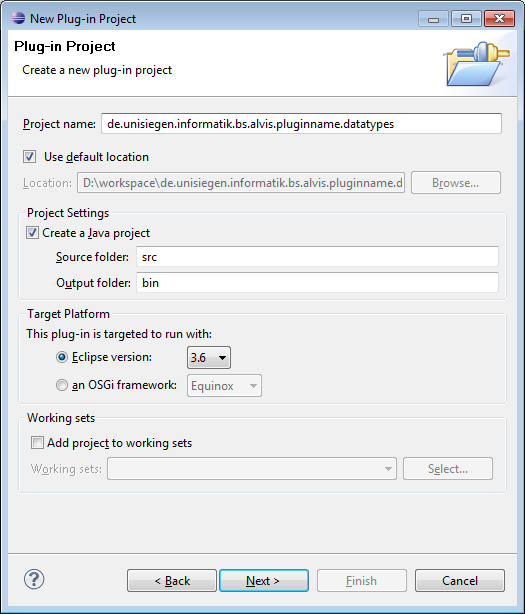
\includegraphics[scale=0.449]{images/new_plugin_datatypes_00}
\\
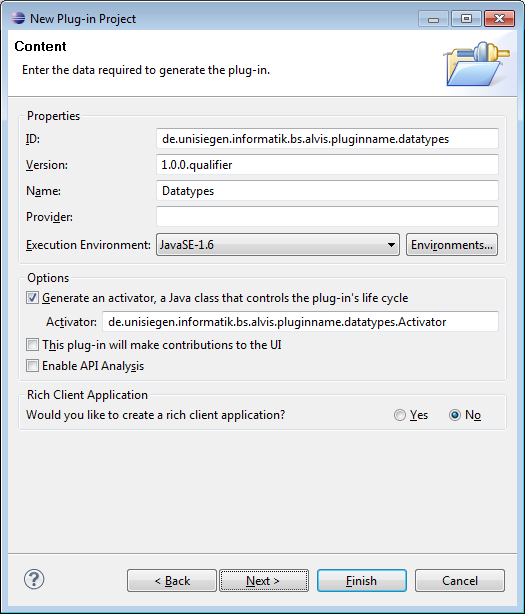
\includegraphics[scale=0.449]{images/new_plugin_datatypes_01}
\end{center}

\subsection{Erstellen von Klassen für Datentypen}
Als nächstes erstelle man für jeden Datentyp eine Klasse \textit{PseudoCodeDatentypname}. Diese Klasse muss von \textit{PCObject} erben.

\lstset{language=java}
\lstinputlisting[caption=Klasse PseudoCodeDatentyp,numbers=left]{sourcecode/PseudoCodeDatentypname.java}

Man implementiere die abstrakten Methoden und überschreibe je nach Bedarf weitere Methoden. Natürlich müssen noch weitere Attribute und Methoden hinzugefügt werden, welche die Logik des Datentypen stellen.
Als Beispiel sehe man sich den Datentypen Graph\footnote{de.unisiegen.informatik.bs.alvis.graph.datatypes.PseudoCodeGraph} aus dem Graph Plugin an. Dieser beinhaltet lediglich Knoten und Kanten. 
Die definierte Schnittstelle\\
\lstinline{public PCObject get(String memberName);}\\
ermöglicht dann den Zugriff auf die Attribute.

\subsection{Erstellen von Interfaces zur graphischen Repräsentation}
Zu diesem Datentyp erstelle man nun ein Interface \textit{GraphicalRepresentationDatentypname}. Dieses Interface muss von \textit{GraphicalRepresentation} erben.

\lstset{language=java}
\lstinputlisting[caption=Interface GraphicalRepresentationDatentyp,numbers=left]{sourcecode/GraphicalRepresentationDatentypname.java}

Dieses Interface wird nachher von der graphischen Repräsentation des neuen Datentyps implementiert. Hier ist es möglich die Schnittstellen zu definieren, welche die graphische Repräsentation auf den reinen Datentypen abbilden. Die graphische Repräsentation eines Datentypen enthält in der Regel noch weitere Metadaten (x- und y-Koordinaten auf dem Bildschirm, Schriftart...). Zum besseren Verständnis sehe man sich hier ebenfalls die Implementierung des Graph Plug-ins an.

\section{\textit{de.unisiegen.informatik.bs.alvis.pluginname}}

Als möchte ich einen Überblick geben, welche verbleibenden Teile in diesem Plug-in zusammengefasst werden.

\begin{enumerate}
\item Für jeden \textbf{Datentyp} wird mindestens eine eigene Klasse erstellt, die diesen Datentyp visualisiert.

\item Es wird ein \textbf{Editor} erstellt, der es ermöglicht ein Beispiel zu erstellen.

\item Es wird ein Klasse erstellt, die den Benutzer nach \textbf{Einstellungen} für den \textbf{Run}\index{Run} fragt.

\item Es wird eine Klasse erstellt, die die \textbf{Visualisierung} der Datentypen im \textbf{Run}-View ermöglicht.

\item Es wird eine Klasse erstellt, die es ermöglicht den momentanen Zustand des Datentyps zu \textbf{exportieren}.

 
\end{enumerate}

Dieses Plug-in beinhaltet Klassen, die das Userinterface erweitern deswegen setzte man dieses mal bei \textit{,,This plug-in will make contributions to the UI''} einen Haken.

\begin{center}
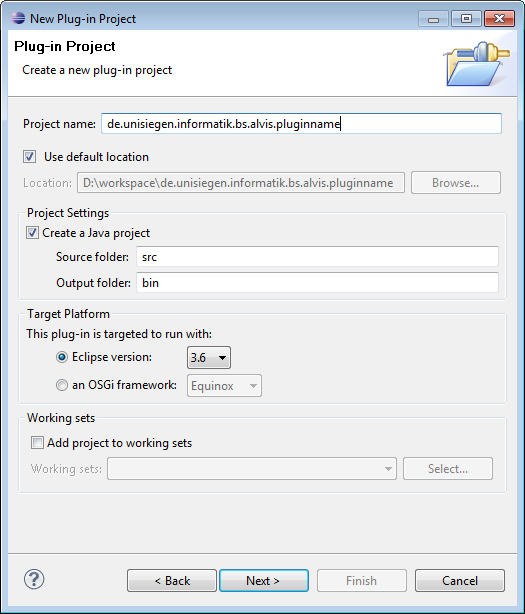
\includegraphics[scale=0.449]{images/new_plugin_datatypes_03}
\\
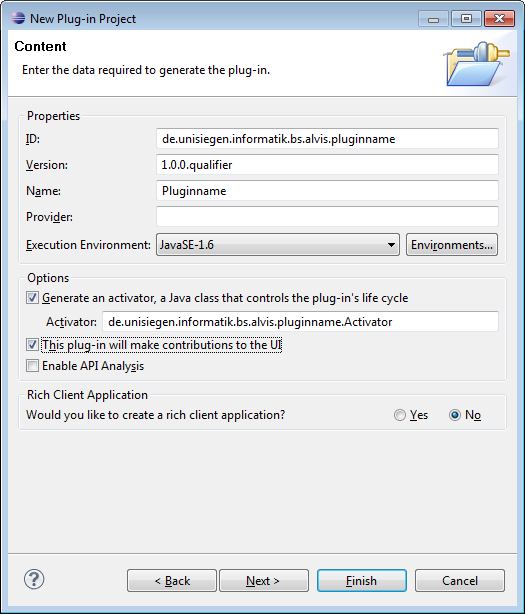
\includegraphics[scale=0.449]{images/new_plugin_datatypes_04}
\end{center}


%%% DATENTYP
%%%
%%%
\subsection{Visualisierung des Datentyps}
Klassen zur Visualisierung des Datentyps wollen wir in das Package \\ \textit{,,de.unisiegen.informatik.bs.alvis.pluginname.graphicalrepresentations''} ablegen.\\ 
\\
Zur Visualisierung von Datentypen benötigt man eine Klasse, welche man an einen Editor oder an einen View hängen kann. Dazu muss diese Klasse einen Konstruktor der Form 
\lstinline{Klasse(Composite parent, ...)} 
haben. Die neue Klasse kann sich dazu aus dem Paket 
,,org.eclipse.swt.widgets\footnote{
\href{http://help.eclipse.org/helios/index.jsp?topic=/org.eclipse.platform.doc.isv/reference/api/org/eclipse/swt/widgets/package-summary.html}{http://help.eclipse.org/helios/index.jsp?topic=/org.eclipse.platform.doc.isv/reference/api/org/eclipse/swt/widgets/package-summary.html}}''
bedienen. \\ 
Damit aus der graphischen Repräsentation  muss die Klasse das von 
\textit{GraphicalRepresentation}\footnote{Siehe dazu: Erstellen von Interfaces zur graphischen Repräsentation} abgeleitetes Interface aus dem Plug-in \\ \textit{,,de.unisiegen.informatik.bs.alvis.pluginname.datatypes''} implementieren.

%%% EDITOR 
%%%
%%%
\subsection{Erstellen eines Editors für ein Beispiel}
Editoren für unser Beispiel wollen wir in das Package \\ \textit{,,de.unisiegen.informatik.bs.alvis.pluginname.editors''} ablegen.\\ 
\\
Wir wollen zum Anlegen und Bearbeiten eines Beispiels einen Editor verwenden. Der Editor speichert unser Beispiel in serialisierter Form in eine Datei. \\
Wir fügen nun in der ,,MANIFEST.MF'' die Extension ,,org.eclipse.ui.editors''  und einen neuen Editor hinzu. \\

\begin{center}
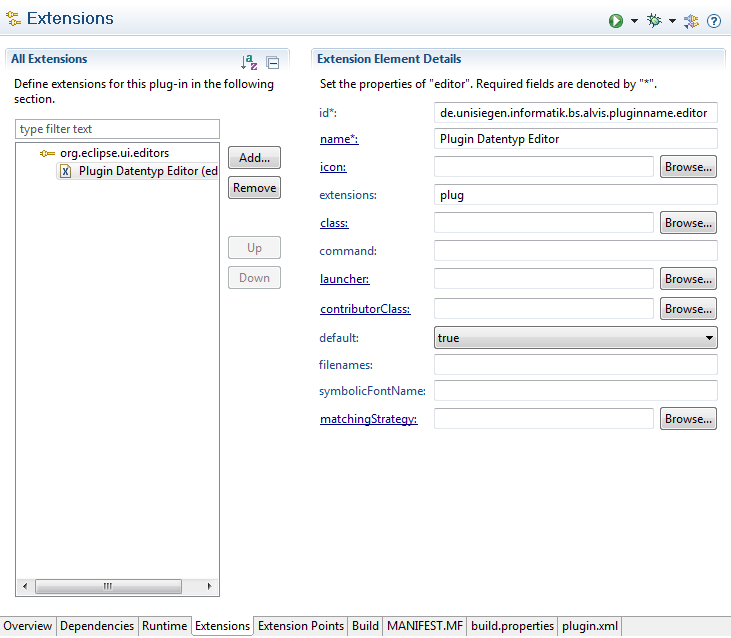
\includegraphics[scale=0.625]{images/new_plugin_editor_00}
\end{center}

Die \textit{id} ist auch hier möglichst aussagekräftig zu wählen.\\
Als \textit{name*:} wähle man einen Namen. Dieser wird als Editor Name angezeigt, wenn man eine Datei per ,,öffnen mit...'' öffnet.\\
\textit{extensions:} ist die Dateiendung (ohne .), für die dieser Editor zuständig ist.\\
\textit{default:} gibt an, ob der Editor der Standard Editor für die Extension ist.\\


Mit einem klick auf \underline{class:} wird die Implementierung für den Editor hinzugefügt.

\begin{center}
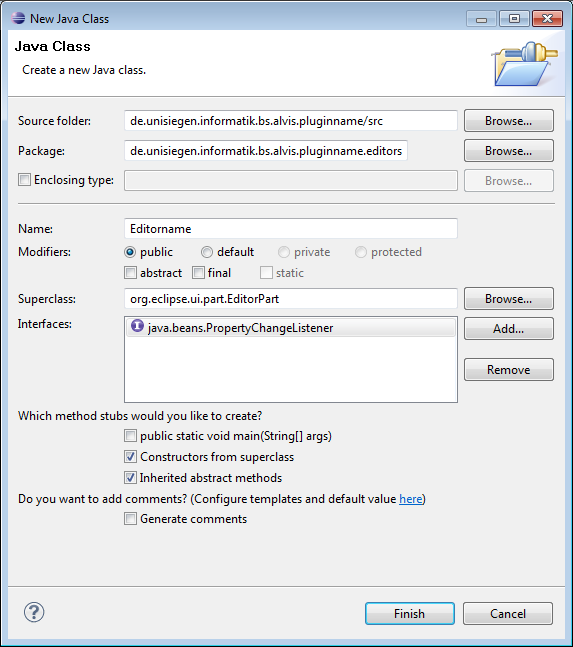
\includegraphics[scale=0.485]{images/new_plugin_editor_01}
\end{center}

Um Ordnung in dem Plugin zu halten erstelle man den Editor im Package \textit{de.unisiegen.informatik.bs.alvis.pluginname.editors}.\\
Weiterhin lässt man den Editor das Interface \textit{PropertyChangeListener} implementieren.\\
Nach einem Klick auf \textit{"Finish"} öffnet sich die Implementierung des Editors. \\

\lstinputlisting[caption=Editor Editorname,numbers=left]{sourcecode/Editorname.java}

Um den Editor zu verstehen stelle man sich vor der Benutzer hätte eine Datei aus dem Package Explorer mit diesem Editor geöffnet. Der Ablauf der Methodenaufrufe sieht dann folgendermaßen aus:\footnote{Mehr Informationen zum Editor unter http://www.ralfebert.de/eclipse\_rcp/editors/}
\begin{enumerate}
\item Der Editor wird per Konstruktor erzeugt.
\item init(IEditorSite, IEditorInput) wird aufgerufen und das für uns interessante IEditorInput Objekt wird übergeben. 
\item createPartControl(Composite) wird aufgerufen und das Parent, dem wir unsere Visualisierungen hinzufügen wird übergeben.
\end{enumerate}

Auf Basis dieses Wissens erweitern wir den Editor um einige Funktionen.
Wir fügen private Attribute hinzu, die die übergebenden Objekte speichern.
In der init-Methode werden einige setMethoden aufgerufen und die privaten Attribute gesetzt.
\\ \\
In der createPartCotrol-Methode wird das Parent gesetzt und eine Methode zum erstellen des Editors aufgerufen.
\\ \\
Die Methode \textit{createEditorFromInput(...)} ist für das laden des Beispiels zuständig. Falls myInput bereits ein gespeichertes Beispiel beinhaltet hat, ist es die Aufgabe dieser Methode den gespeicherten Zustand des Beispiels wieder herzustellen. Falls die Datei frisch erstellt wurde so muss diese Methode einen leeren Editor Zustand herstellen.
\\ \\
Die \textit{doSave}-Methode serialisiert\footnote{Es wird empfohlen http://xstream.codehaus.org/ zum Serialisieren zu verwenden. } den derzeitigen Zustand des Editors in die geöffnete Datei.

\lstinputlisting[caption=Editor Editorname erweitert,numbers=left]{sourcecode/Editorname_extends.java}

\subsection{Registrieren eines Wizards}
Damit der Benutzer auch eine Möglichkeit hat Dateien des neuen Typs anzulegen benötigt man einen \textbf{Wizard} für diese Dateiendung. Ein Wizard ist ein Dialog, der es dem Benutzer ermöglicht Dateien eines bestimmten Typs anzulegen. Dieser muss die Extension \textit{,,org.eclipse.ui.newWizards''} bedienen.

\subsection{Visualisierung des Runs}
Wenn der Benutzer den Algorithmus und sein Beispiel definiert hat und einen Run startet wird nach Plug-ins gesucht, die die Extension ,,de.unisiegen.informatik.bs.alvis.runvisualizer'' erweitern. Diesen Plug-ins werden dann alle Datentypen und das Parent herunter gegeben. Das Plug-in prüft dann, ob es sich bei einem der Datentypen um einen Datentyp des Plug-ins handelt und hängt dann die Visualisierung seiner Datentypen an das Parent.
\\
Diesen Extension Point wollen wir nun in unserem Plug-in erweitern.
\\
Dazu öffnen wir als nächstes die ,,MANIFEST.MF'' in unserem Plug-in und fügen eine ,,Dependencie'' zu ,,de.unisiegen.informatik.bs.alvis'' hinzu. Danach wählen den Reiter ,,Extensions'' aus. 

Wir fügen den Extension Point ,,de.unisiegen.informatik.bs.alvis.runvisualizer'' aus dem Plug-in  ,,de.unisiegen.informatik.bs.alvis'' hinzu. 

Mit der rechten Maustaste auf den neu hinzugefügten Extension Point lässt sich unter ,,New'' ein neuer ,,RunVisulizer'' hinzufügen.

\begin{center}
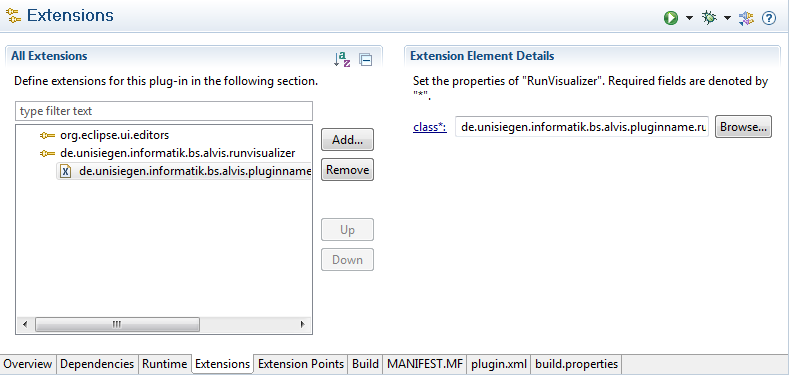
\includegraphics[scale=0.58]{images/new_plugin_runvisualizer_01}
\end{center}

Der Link ,,\textit{class*:}'' ermöglicht es uns eine neue Klasse anzulegen, die folgende Anforderungen erfüllt.

\begin{center}
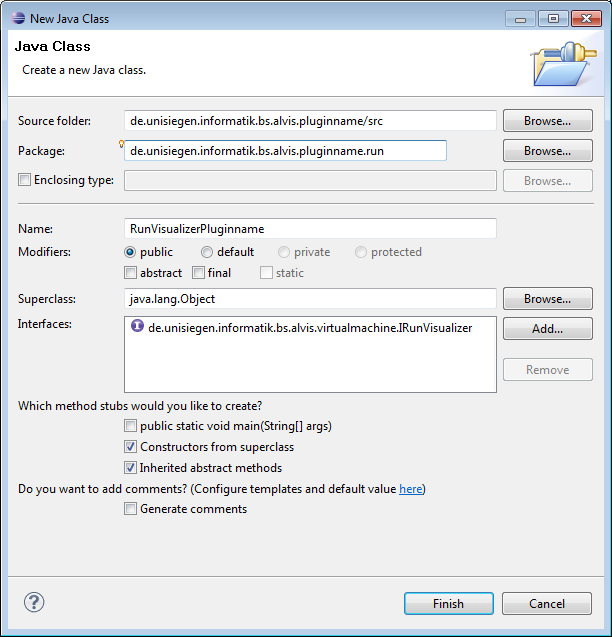
\includegraphics[scale=0.478]{images/new_plugin_runvisualizer_00}
\end{center}

Wir bestätigen die Einstellungen mit einem Klick auf ,,Finish'' und erhalten eine Klasse mit folgendem Inhalt.

\lstinputlisting[caption=Klasse RunVisualizerPluginname,numbers=left]{sourcecode/RunVisualizerPluginname.java}

Hier gehen wir genau so vor, wie wir es schon bei der Load-Methode des Editors gemacht haben.

\subsection{Datentypen registrieren}

Als letztes muss unser Plug-in den anderen Plug-ins noch mitteilen können, welche Datentypen es beinhaltet. Dafür gibt es natürlich auch wieder eine definierte Schnittstelle.
\\ \\
Wir öffnen die ,,MANIFEST.MF'' und fügen die Extension \\ ,,de.unisiegen.informatik.bs.alvis.extensionpoints.datatypelist'' hinzu. Wir wählen ,,New'' \(\rightarrow\) ,,DatatypeList'' und klicken den Link ,,\underline{class*:}''.
\\ \\
Als nächstes öffnet sich ein neues Fenster, dass uns anbietet eine neue Klasse anzulegen. Wir legen die Klasse in das Package \\,,de.unisiegen.informatik.bs.alvis.pluginname.datatypes''.

\begin{center}
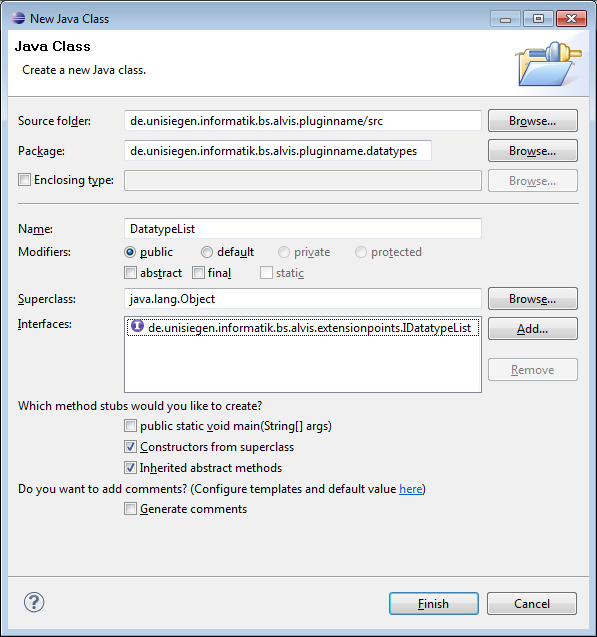
\includegraphics[scale=0.48]{images/new_plugin_datatypeslist_00}
\end{center}

Anschließend bestätigen wir mit ,,Finish'' werfen einen Blick auf die Implementierung.
Sollte Eclipse sich über fehlende Methoden beschweren, so kann man den Mauszeiger über den Klassennamen halten und auf das Kontext Menü warten. Anschließend lassen sich die fehlenden Methoden mit einem Klick auf den Link ,,\textit{Add unimplemented methods}'' hinzufügen.

\begin{center}
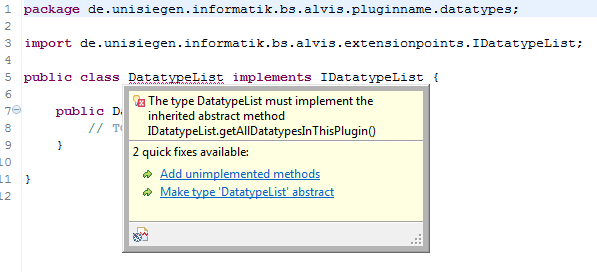
\includegraphics[scale=0.48]{images/new_plugin_datatypeslist_01}
\end{center}

Wir wollen sichergehen, dass der Import von PCObject\footnote{de.unisiegen.informatik.bs.alvis.primitive.datatypes.PCObject} funktionieren. Wir ändern auf ,,de.unisiegen.informatik.bs.alvis.primitive.datatypes.PCObject''. Und fügen ,,de.unisiegen.informatik.bs.alvis.primitive.datatypes'' via ,,Add ... to imported packages'' zu den ,,Imported packages'' hinzufügen.


\begin{center}
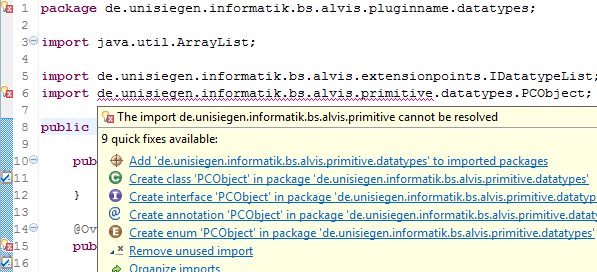
\includegraphics[scale=0.48]{images/new_plugin_datatypeslist_02}
\end{center}

Danach sollte die Klasse in etwa so aussehen.
\lstinputlisting[caption=Klasse DatatypeList,numbers=left]{sourcecode/DatatypeList.java}

Nun wollen wir noch die Methode \textit{getAllDatatypesInThisPlugin()} implementieren.
In dieser Methode geben wir ein Null-Object von jedem Datentyp den wir erstellt haben in einer ArrayList zurück.
\lstinputlisting[caption=Klasse DatatypeList,numbers=left]{sourcecode/DatatypeList_01.java}


\section{Anhang}
In diesem Anhang möchte ich noch auf ein paar Dinge aufmerksam machen, die uns bei der Arbeit mit RCP einiges an Zeit gekostet haben, eigentlich aber recht simpel zu lösen waren.
\subsection{Der Klabautermann}
Es kam vor, dass das Projekt einfach nicht gestartet ist, obwohl das Projekt frisch ausgecheckt wurde. Das Projekt lief auf dem einen PC und auf dem anderen PC nicht. Man wird nach 300 Stunden mit RCP abergläubig, aber wir sind uns sicher, dass das Problem eine Ursache hat: \\
Der Klabautermann ist in deinem Workspace und treibt dort sein Unwesen.\\
\\
Wenn du festgestellt hast, dass der Klabautermann in deinem Workspace sein Unwesen treibt...
\begin{itemize}
\item markiere alle Plugins, klicke dann dann auf ,,Project'',  dann auf ,,Clean...''.
\item starte Eclipse neu.
\item refresh den Workspace indem du alle Plugins markierst und ,,F5'' drückst.  
\end{itemize}
\subsection{Probleme beim Start}
Hast du beim Start des Projekts Probleme kann dir vielleicht eine der folgenden Lösungen helfen.

\subsubsection{Fehlende Plugins}
Wird beim Start hingewiesen, dass Plugins fehlen, dann Wähle ,,Run'' -> ,,Run Configurations...''. Es öffnet sich ein neues Fenster. Es kommt vor, dass nicht alle Buttons sichtbar sind. Ziehe das Fenster so groß wie nötig um alle Elemente zu sehen. Anschließend wählst du im linken Teil des Fensters unter ,,Eclipse Application'' die Application die du starten möchtest. Anschließend klickst du auf der rechten Seite auf den Reiter ,,Plug-ins'' und drückst den Button ,,Add Required Plug-ins''. 
\subsubsection{.jar Dateien einbinden}
Um externe .jar Dateien in ein Plugin einzubinden darf man nicht, wie sonst in Java üblich, das jar einfach zum Build Path hinzufügen, sondern man muss es in der MANIFEST.MF unter ,,Runtime'' unter ,,Classpath'' einbinden.

\printindex
\end{document}